\documentclass{standalone}

\usepackage[dvipsnames]{xcolor}
\usepackage{tikz}

\begin{document}

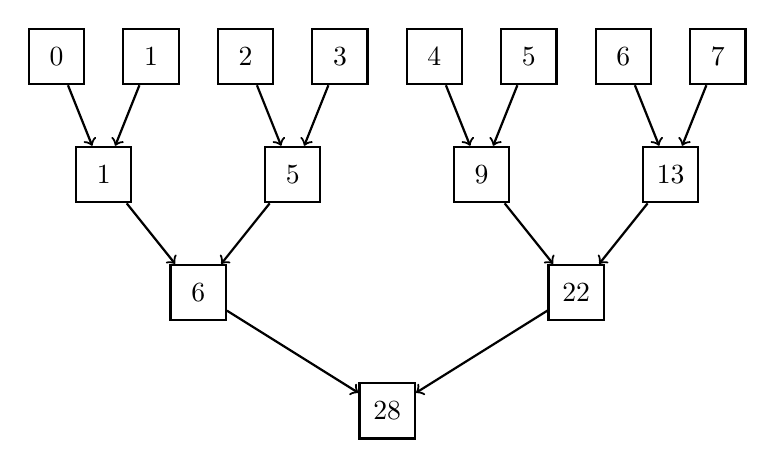
\begin{tikzpicture}[thick]
  \tikzset{box/.style={draw, rectangle, inner sep=10pt}}

  \foreach \i in {0, 1, ..., 7} {
    \path ({\i * 1.2}, 0) coordinate [box] (0-\i) node {\i};
  }

  \foreach \i/\v in {0/1, 1/5, 2/9, 3/13} {
    \path ({0.6 + \i * 2.4}, -1.5) coordinate [box] (1-\i) node {\v};
  }

  \foreach \i/\v in {0/6, 1/22} {
    \path ({1.8 + \i * 4.8}, -3) coordinate [box] (2-\i) node {\v};
  }

  \path (4.2, -4.5) coordinate [box] (final) node {28};

  % Edges
  \draw [->] (0-0) -- (1-0);
  \draw [->] (0-1) -- (1-0);
  \draw [->] (0-2) -- (1-1);
  \draw [->] (0-3) -- (1-1);
  \draw [->] (0-4) -- (1-2);
  \draw [->] (0-5) -- (1-2);
  \draw [->] (0-6) -- (1-3);
  \draw [->] (0-7) -- (1-3);

  \draw [->] (1-0) -- (2-0);
  \draw [->] (1-1) -- (2-0);
  \draw [->] (1-2) -- (2-1);
  \draw [->] (1-3) -- (2-1);

  \draw [->] (2-0) -- (final);
  \draw [->] (2-1) -- (final);

\end{tikzpicture}

\end{document}
